
\documentclass{article}[14pt]
\usepackage{multicol, enumerate, enumitem, hyperref, color, soul, setspace, parskip, fancyhdr, amssymb, amsthm, amsmath, bbm, latexsym, units, mathtools}
\everymath{\displaystyle}
\usepackage[headsep=0.5cm,headheight=0cm, left=1 in,right= 1 in,top= 1 in,bottom= 1 in]{geometry}
\pagestyle{fancy}
\lhead{}
\chead{Answer Key for Module\,6\,-\,Polynomial\,Functions Version A}
\rhead{}
\lfoot{Summer\,C\,2020}
\cfoot{}
\rfoot{}
\begin{document}
\textbf{This key should allow you to understand why you choose the option you did (beyond just getting a question right or wrong). \href{https://xronos.clas.ufl.edu/mac1105spring2020/courseDescriptionAndMisc/Exams/LearningFromResults}{More instructions on how to use this key can be found here}.}

\textbf{If you have a suggestion to make the keys better, \href{https://forms.gle/CZkbZmPbC9XALEE88}{please fill out the short survey here}.}

\textit{Note: This key is auto-generated and may contain issues and/or errors. The keys are reviewed after each exam to ensure grading is done accurately. If there are issues (like duplicate options), they are noted in the offline gradebook. The keys are a work-in-progress to give students as many resources to improve as possible.}

\rule{\textwidth}{0.4pt}

26. Describe the end behavior of the polynomial below.
$$ f(x) = -7(x - 8)^{2}(x + 8)^{5}(x - 7)^{4}(x + 7)^{5} $$ 

 
 The solution is  
 \begin{center} 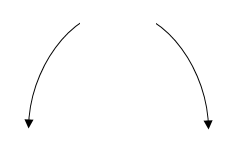
\includegraphics[width=0.3\textwidth]{../Figures/endBehaviorNegativeEvenA.png} \end{center}\begin{tabular}{|c|c|} 
\hline 
 & \tabularnewline 
 \textbf{A.} 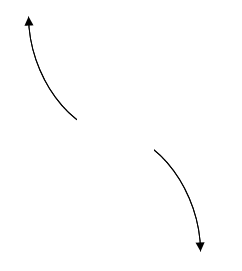
\includegraphics[width=0.3\textwidth]{../Figures/endBehaviorNegativeOddA.png} & \textbf{B.} 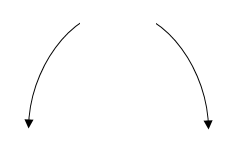
\includegraphics[width=0.3\textwidth]{../Figures/endBehaviorNegativeEvenA.png} \tabularnewline 
\hline 
 & \tabularnewline 
 \textbf{C.} 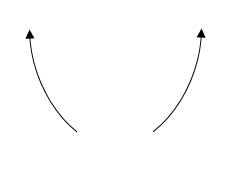
\includegraphics[width=0.3\textwidth]{../Figures/endBehaviorPositiveEvenA.png} & \textbf{D.} 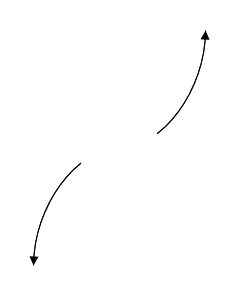
\includegraphics[width=0.3\textwidth]{../Figures/endBehaviorPositiveOddA.png} \tabularnewline 
\hline 
 E. None of the figures above. & \tabularnewline 
\hline 
 \end{tabular} 
 
\textbf{General Comments:} Remember that end behavior is determined by the leading coefficient AND whether the \textbf{sum} of the multiplicities is positive or negative.

-----------------------------------------------

27. Construct the lowest-degree polynomial given the zeros below. Then, choose the intervals that contain the coefficients of the polynomial in the form $x^3+bx^2+cx+d$.
$$ 4 - 2i \text{ and } 4 $$ 
The solution is $ x^{3} -12 x^{2} +52 x -80 $ 

\begin{enumerate}[label=\Alph*.] 
\item $ b \in [-2, 2], c \in [-12, -6], \text{ and } d \in [15, 19] $ 

 $x^{3} + x^{2} -8 x + 16$, which corresponds to multiplying out $(x -4)(x -4)$. 
\item $ b \in [5, 17], c \in [44, 60], \text{ and } d \in [79, 89] $ 

 $x^{3} +12 x^{2} +52 x + 80$, which corresponds to multiplying out $(x-(4 - 2i))(x-(4 + 2i))(x + 4)$. 
\item $ b \in [-2, 2], c \in [-7, 2], \text{ and } d \in [-12, -5] $ 

 $x^{3} + x^{2} -2 x -8$, which corresponds to multiplying out $(x + 2)(x -4)$. 
\item $ b \in [-19, -9], c \in [44, 60], \text{ and } d \in [-83, -74] $ 

 * $x^{3} -12 x^{2} +52 x -80$, which is the correct option. 
\item $ \text{None of the above.} $ 

 This corresponds to making an unanticipated error or not understanding how to use nonreal complex numbers to create the lowest-degree polynomial. If you chose this and are not sure what you did wrong, please contact the coordinator for help. 
\end{enumerate} 
 
General Comments: Remember that the conjugate of $a+bi$ is $a-bi$. Since these zeros always come in pairs, we need to multiply out $(x-(4 - 2i))(x-(4 + 2i))(x-(4))$.

-----------------------------------------------

28. Which of the following equations \textit{could} be of the graph presented below?
\begin{center} 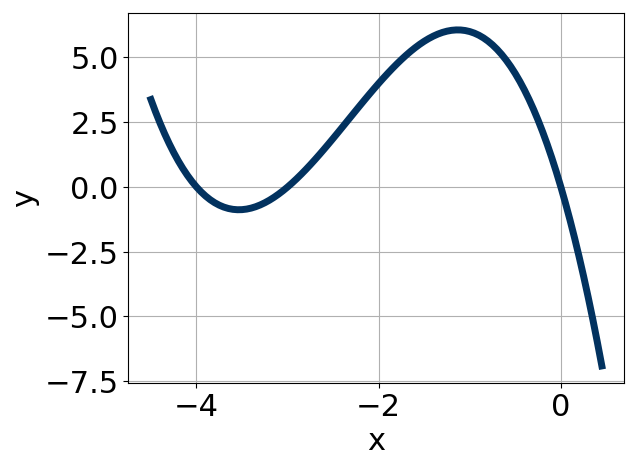
\includegraphics[width=0.3\textwidth]{../Figures/polyGraphToFunctionA.png} \end{center} 

The solution is $ 2(x - 1)^{6} (x + 4)^{8} (x + 3)^{5} $ 

\begin{enumerate}[label=\Alph*.] 
\item $ 3(x - 1)^{4} (x + 4)^{7} (x + 3)^{11} $ 

 The factor $(x + 4)$ should have an even power. 
\item $ 2(x - 1)^{6} (x + 4)^{8} (x + 3)^{5} $ 

 * This is the correct option. 
\item $ 16(x - 1)^{6} (x + 4)^{5} (x + 3)^{10} $ 

 The factor $(x + 4)$ should have an even power and the factor $(x + 3)$ should have an odd power. 
\item $ -17(x - 1)^{8} (x + 4)^{8} (x + 3)^{10} $ 

 The factor $(x + 3)$ should have an odd power and the leading coefficient should be the opposite sign. 
\item $ -13(x - 1)^{8} (x + 4)^{4} (x + 3)^{11} $ 

 This corresponds to the leading coefficient being the opposite value than it should be. 
\end{enumerate} 
 
General Comments: Draw the x-axis to determine which zeros are touching (and so have even multiplicity) or cross (and have odd multiplicity).

-----------------------------------------------

29. Construct the lowest-degree polynomial given the zeros below. Then, choose the intervals that contain the coefficients of the polynomial in the form $ax^3+bx^2+cx+d$.
$$ -2, -3, \text{ and } \frac{2}{5} $$ 
The solution is $ 5x^{3} +23 x^{2} +20 x -12 $ 

\begin{enumerate}[label=\Alph*.] 
\item $ a \in [3, 6], b \in [22.5, 25.8], c \in [18, 22], \text{ and } d \in [8, 19] $ 

 $5x^{3} +23 x^{2} +20 x + 12$, which corresponds to multiplying everything correctly except the constant term. 
\item $ a \in [3, 6], b \in [-28.1, -24.8], c \in [37, 45], \text{ and } d \in [-13, -8] $ 

 $5x^{3} -27 x^{2} +40 x -12$, which corresponds to multiplying out $(x + 1)(x + 1)(5x -5)$. 
\item $ a \in [3, 6], b \in [-26.2, -20.1], c \in [18, 22], \text{ and } d \in [8, 19] $ 

 $5x^{3} -23 x^{2} +20 x + 12$, which corresponds to multiplying out $(x -2)(x -3)(5x + 2)$. 
\item $ a \in [3, 6], b \in [22.5, 25.8], c \in [18, 22], \text{ and } d \in [-13, -8] $ 

 * $5x^{3} +23 x^{2} +20 x -12$, which is the correct option. 
\item $ a \in [3, 6], b \in [0.9, 6.3], c \in [-39, -23], \text{ and } d \in [8, 19] $ 

 $5x^{3} +3 x^{2} -32 x + 12$, which corresponds to multiplying out $(x + 1)(x -1)(5x -5)$. 
\end{enumerate} 
 
General Comments: To construct the lowest-degree polynomial, you want to multiply out $(x + 2)(x + 3)(5x -2)$

-----------------------------------------------

30. Describe the zero behavior of the zero $x = 2$ of the polynomial below.
$$ f(x) = -5(x - 6)^{10}(x + 6)^{9}(x - 2)^{8}(x + 2)^{7} $$ 

 
 The solution is  
 \begin{center} 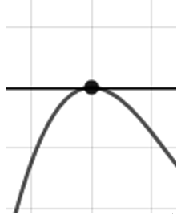
\includegraphics[width=0.3\textwidth]{../Figures/zeroBehaviorNegativeEvenA.png} \end{center}\begin{tabular}{|c|c|} 
\hline 
 & \tabularnewline 
 \textbf{A.} 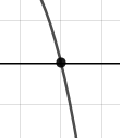
\includegraphics[width=0.3\textwidth]{../Figures/zeroBehaviorNegativeOddA.png} & \textbf{B.} 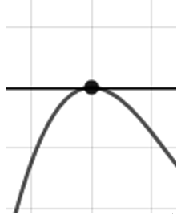
\includegraphics[width=0.3\textwidth]{../Figures/zeroBehaviorNegativeEvenA.png} \tabularnewline 
\hline 
 & \tabularnewline 
 \textbf{C.} 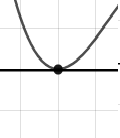
\includegraphics[width=0.3\textwidth]{../Figures/zeroBehaviorPositiveEvenA.png} & \textbf{D.} 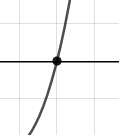
\includegraphics[width=0.3\textwidth]{../Figures/zeroBehaviorPositiveOddA.png} \tabularnewline 
\hline 
 E. None of the figures above. & \tabularnewline 
\hline 
 \end{tabular} 
 
\textbf{General Comments:} You will need to sketch the entire graph, then zoom in on the zero the question asks about.

-----------------------------------------------


\end{document}

